\documentclass{article}

\usepackage{authblk}
\usepackage{amsmath}
\usepackage{amsfonts}
\usepackage{amssymb}
\usepackage{amsthm}
\usepackage{graphicx}

\title{\textbf{Computational Biology: Project 2 Report}}

\author[1]{Haoyu Zhao 2016012390;
  Lukai Li 2015012202;
  Yi Dai 2015012204}
\date{}

\begin{document}
\maketitle
\clearpage

\section{Introduction}
\textbf{Acknowledgement:} In this project, Haoyu Zhao came up with an idea that slightly change the k-means clustering algorithm and apply it into this project. He doesn't know whether this method has already been published and he doesn't know whether this small change can improve the performance or get more things useful in this project. He will present the result in this report and try to illustrate the change. He will also discuss the method in the class presentation and discuss whether the change does some meaningful things.\par

In this project, we use 2 method to cluster.\\
~\\
The first is to eliminate the clustering centers(`principal component') of each image and then clustering. Then eliminate the projection on the clustering centers of the previous 2 clustering phases and then clustering.\\
~\\
The second is to eliminate the projection of the data on the subspace generated by all the clustering centers in the previous phase of the clustering and then iterate for some time.\\
~\\
We provide all the image result of these 2 version of the algorithm but we only keep the code for the second version of clustering algorithm. It is easy to change the second verison of clustering algorithm into the first kind of our algorithm.\\
~\\
We think that our first algorithm performs better but the second version can run faster.\\
~\\
The image of the output of the first verison of the algorithm is stored in the ./code/test1/\\

\section{Flow Chart of Algorithm}
First version of our algorithm\\
~\\
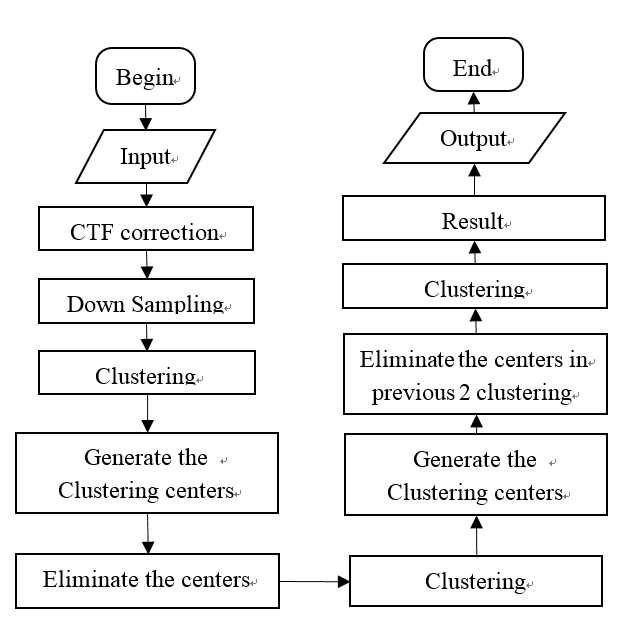
\includegraphics[width=4.8in]{111}
~\\
Second version of our algorithm\\
~\\
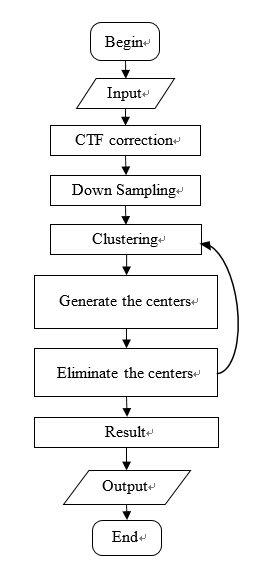
\includegraphics[width=3in]{123}

\section{Details of Algorithm}
\subsection{CTF Correction and Down Sampling}

First we do the CTF correction for each of the graph. The parameters can be obtained from the .star file and the CTF function is
\begin{equation*}
	CTF(s,\theta) = -\left(\sqrt{1 - Q^2}sin\gamma(s,\theta) + Qcos\gamma(s,\theta)\right).
\end{equation*}
where
\begin{equation*}
	\gamma(s,\theta) = 2\pi \left(-\frac{C_s\lambda^3s^4}{4} + \frac{\triangle z(\theta)\lambda s^2}{2}\right)
\end{equation*}
and
\begin{equation*}
	\triangle z(\theta) = \triangle z_0 + \triangle z_1cos(2(\theta - \theta_0)).
\end{equation*}
~\\
\par
We use the phase flipping to do the ctf correction. We first do the 2-dimentional Fast Fourier Transformation to the original graph, and then divide the 2dfft transformed graph by the absolute value of the ctf correction function. Then we use the inverse transformation of the 2-d fast fourier transformation to get the ctf corrected graph.\par
Then because of the computational resources, we do the down sampling. We first select the cells out by an 160 by 160 pixels image, and we do the mean pooling to each 2 by 2 block and we finally get the 80 by 80 cell images. We rescale the image by a constant in order to see the distance result clearly in the measurement.
\subsection{First Clustering}
	We first use the k-means algorithm to do the clustering. We set the nubmer of the initial number of clusters to 25 and we eliminate the clusters that have less then 100(or 75) to avoid from some outliers. Then we add the image in the same class up and get the center of each of the clusters. We save the images and then save the centers of the clustering 
\subsection{Second(or Third) Clustering}
	From the first clustering we get the centers of each clusters. We find that after the first clustering, many clustering are actually the same. The only different is that the images rotate for some angle. And to let each of the clusters has enough images, we cannot enlarge the initial number of the clusters. So what we do is just eliminate the features that clustered from the first clustering and just do another clustering.\par
	In the elemination of the clustering, we first try to eliminate each of the images just by its class centers, that is for $x^{(i)}$ that have the center $\mu^{(i)}$, we change
	\begin{equation}\label{vec}
		x^{(i)} \leftarrow x^{(i)} - \frac{\mu^{(i)}}{\mid \mu^{(i)}\mid^2}\cdot \mu^{(i)T}x^{(i)}
	\end{equation}
and then use the kmeans clustering to do the second cluster. We denote this by eliminate the centers of each of the class.\\
~\\
We also develop another kind of feature eliminating process that is we eliminate the whole subspace generated by all of the centers. Suppose that the matrix of the images is
\begin{equation*}
	X = \left[
	\begin{aligned}
		-&x^{(1)T}-\\
		-&x^{(2)T}-\\
		-&x^{(3)T}-\\
		-&\dots-\\
		-&x^{(n)T}-
	\end{aligned}\right]
\end{equation*}
and the centers matrix is
\begin{equation*}
	\Sigma = \left[
	\begin{aligned}
	-&\mu^{(1)T}-\\
	-&\mu^{(2)T}-\\
	-&\mu^{(3)T}-\\
	-&\dots-\\
	-&\mu^{(n)T}-
	\end{aligned}\right]
\end{equation*}
Then the new data matrix for clustering is
\begin{equation}\label{space}
	X_0 = X - (\Sigma^T(\Sigma\Sigma^T)^{-1}\Sigma X^T).
\end{equation}
Then we do the second(or third) clustering using the eliminated subspaced(or center of class) data.\par
We can actually clustering using many ways of eleminating the subspaced data. We can eliminate each clustering center, we can eliminate the subspace generated by the last time clustering centers, as equation (\ref{space})(we do this in the project), and we can eliminate the centers in each examples(equation (\ref{vec})) as an alternating method.

\subsection{Measurement}
There are 2 ways to measure the algorithm and the performance.\par The first is to just look at the clustered images and see whether the images make sense.\par
The second is to compute the sum of the squared distance from each of the image to its centers. We know that it is just the cost function of the k-means algorithm. For those clusters that we eliminate, we do not calculate the squared distance of them. We first take the mean of the squared distance in each of the clusters and then average them for the number of the clusters.


\section{Final Result and Performance Evaluation}
In this section we will present some tests of different implementations. We will just present the images for all test and we will present the images and the mean of the squared distance of the final implementation.\par

These are the test images for the k-means algorithm, for initial clusters numbers are 16 and 36.\\
~\\
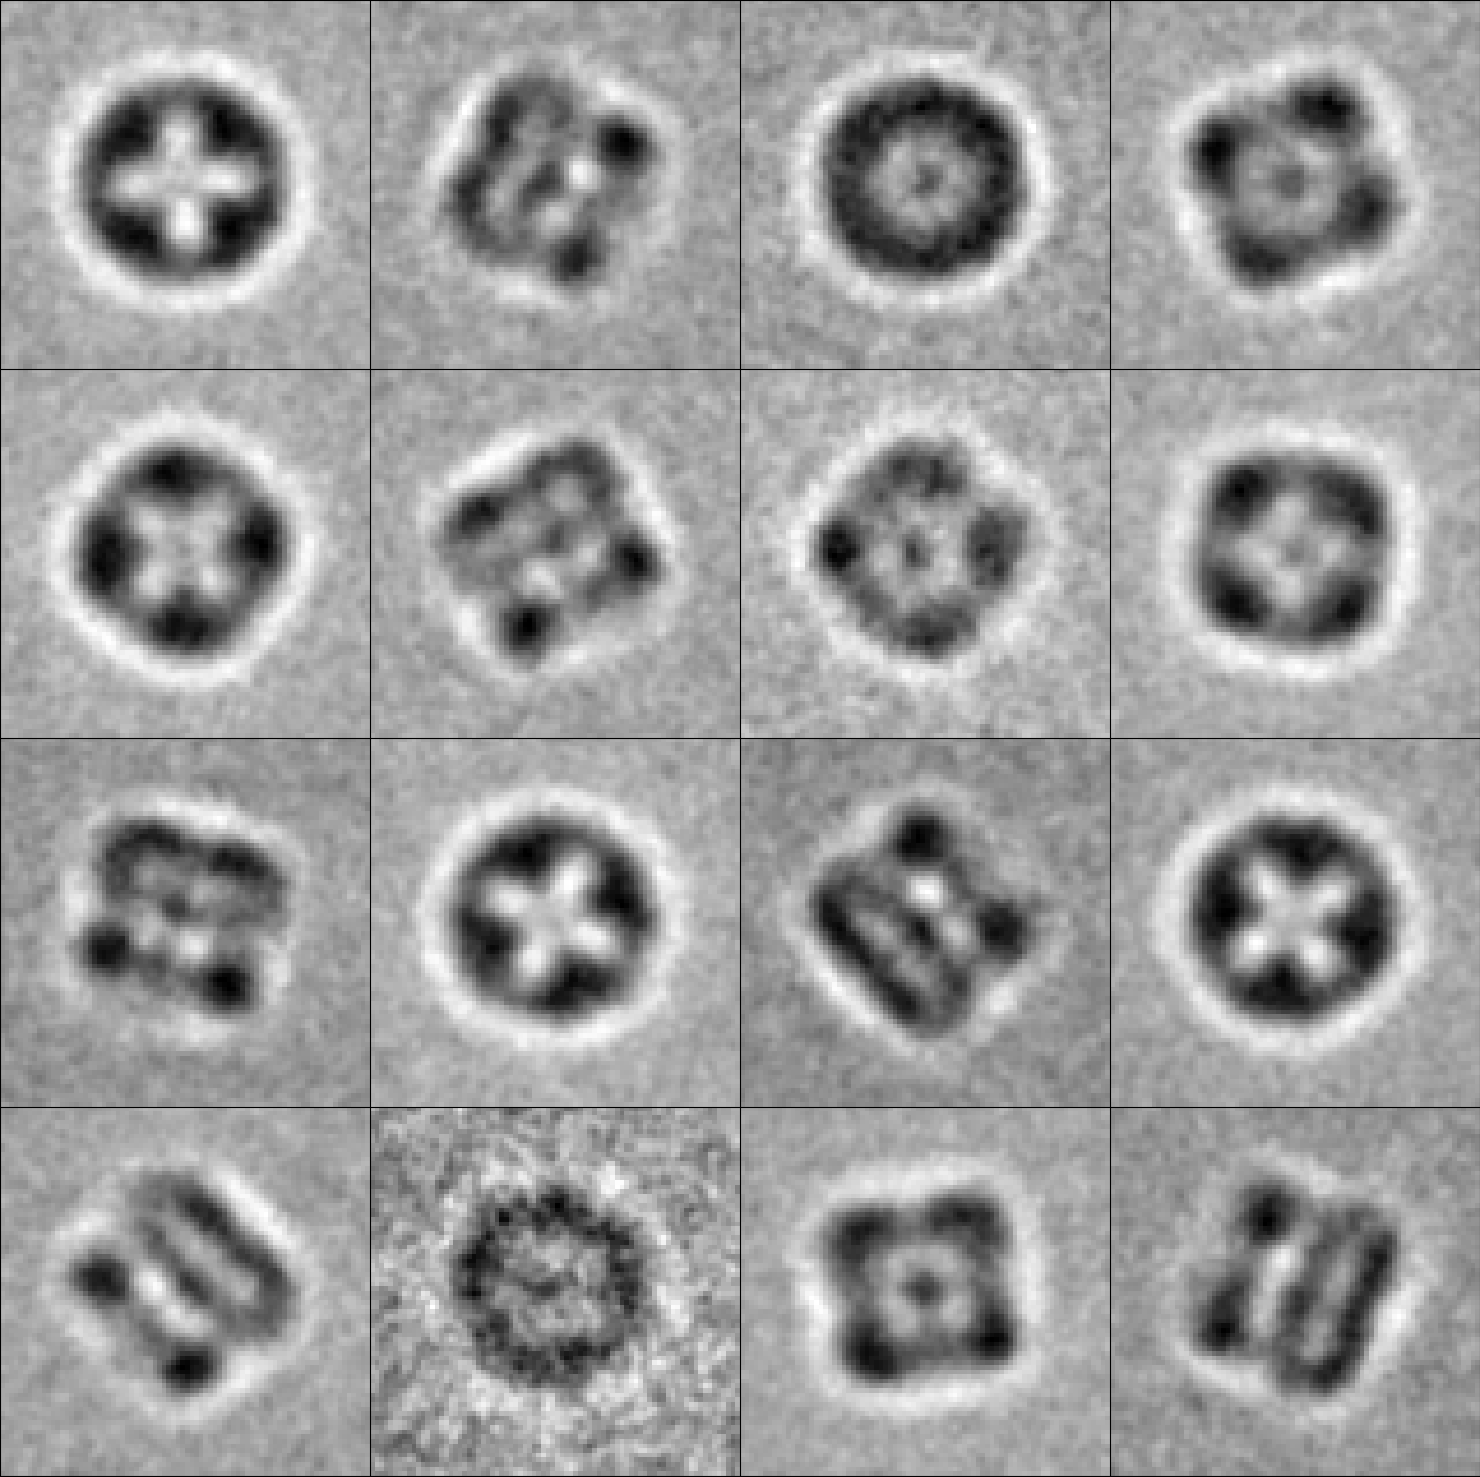
\includegraphics[width=4.8in]{raw_kmeans_16}
~\\
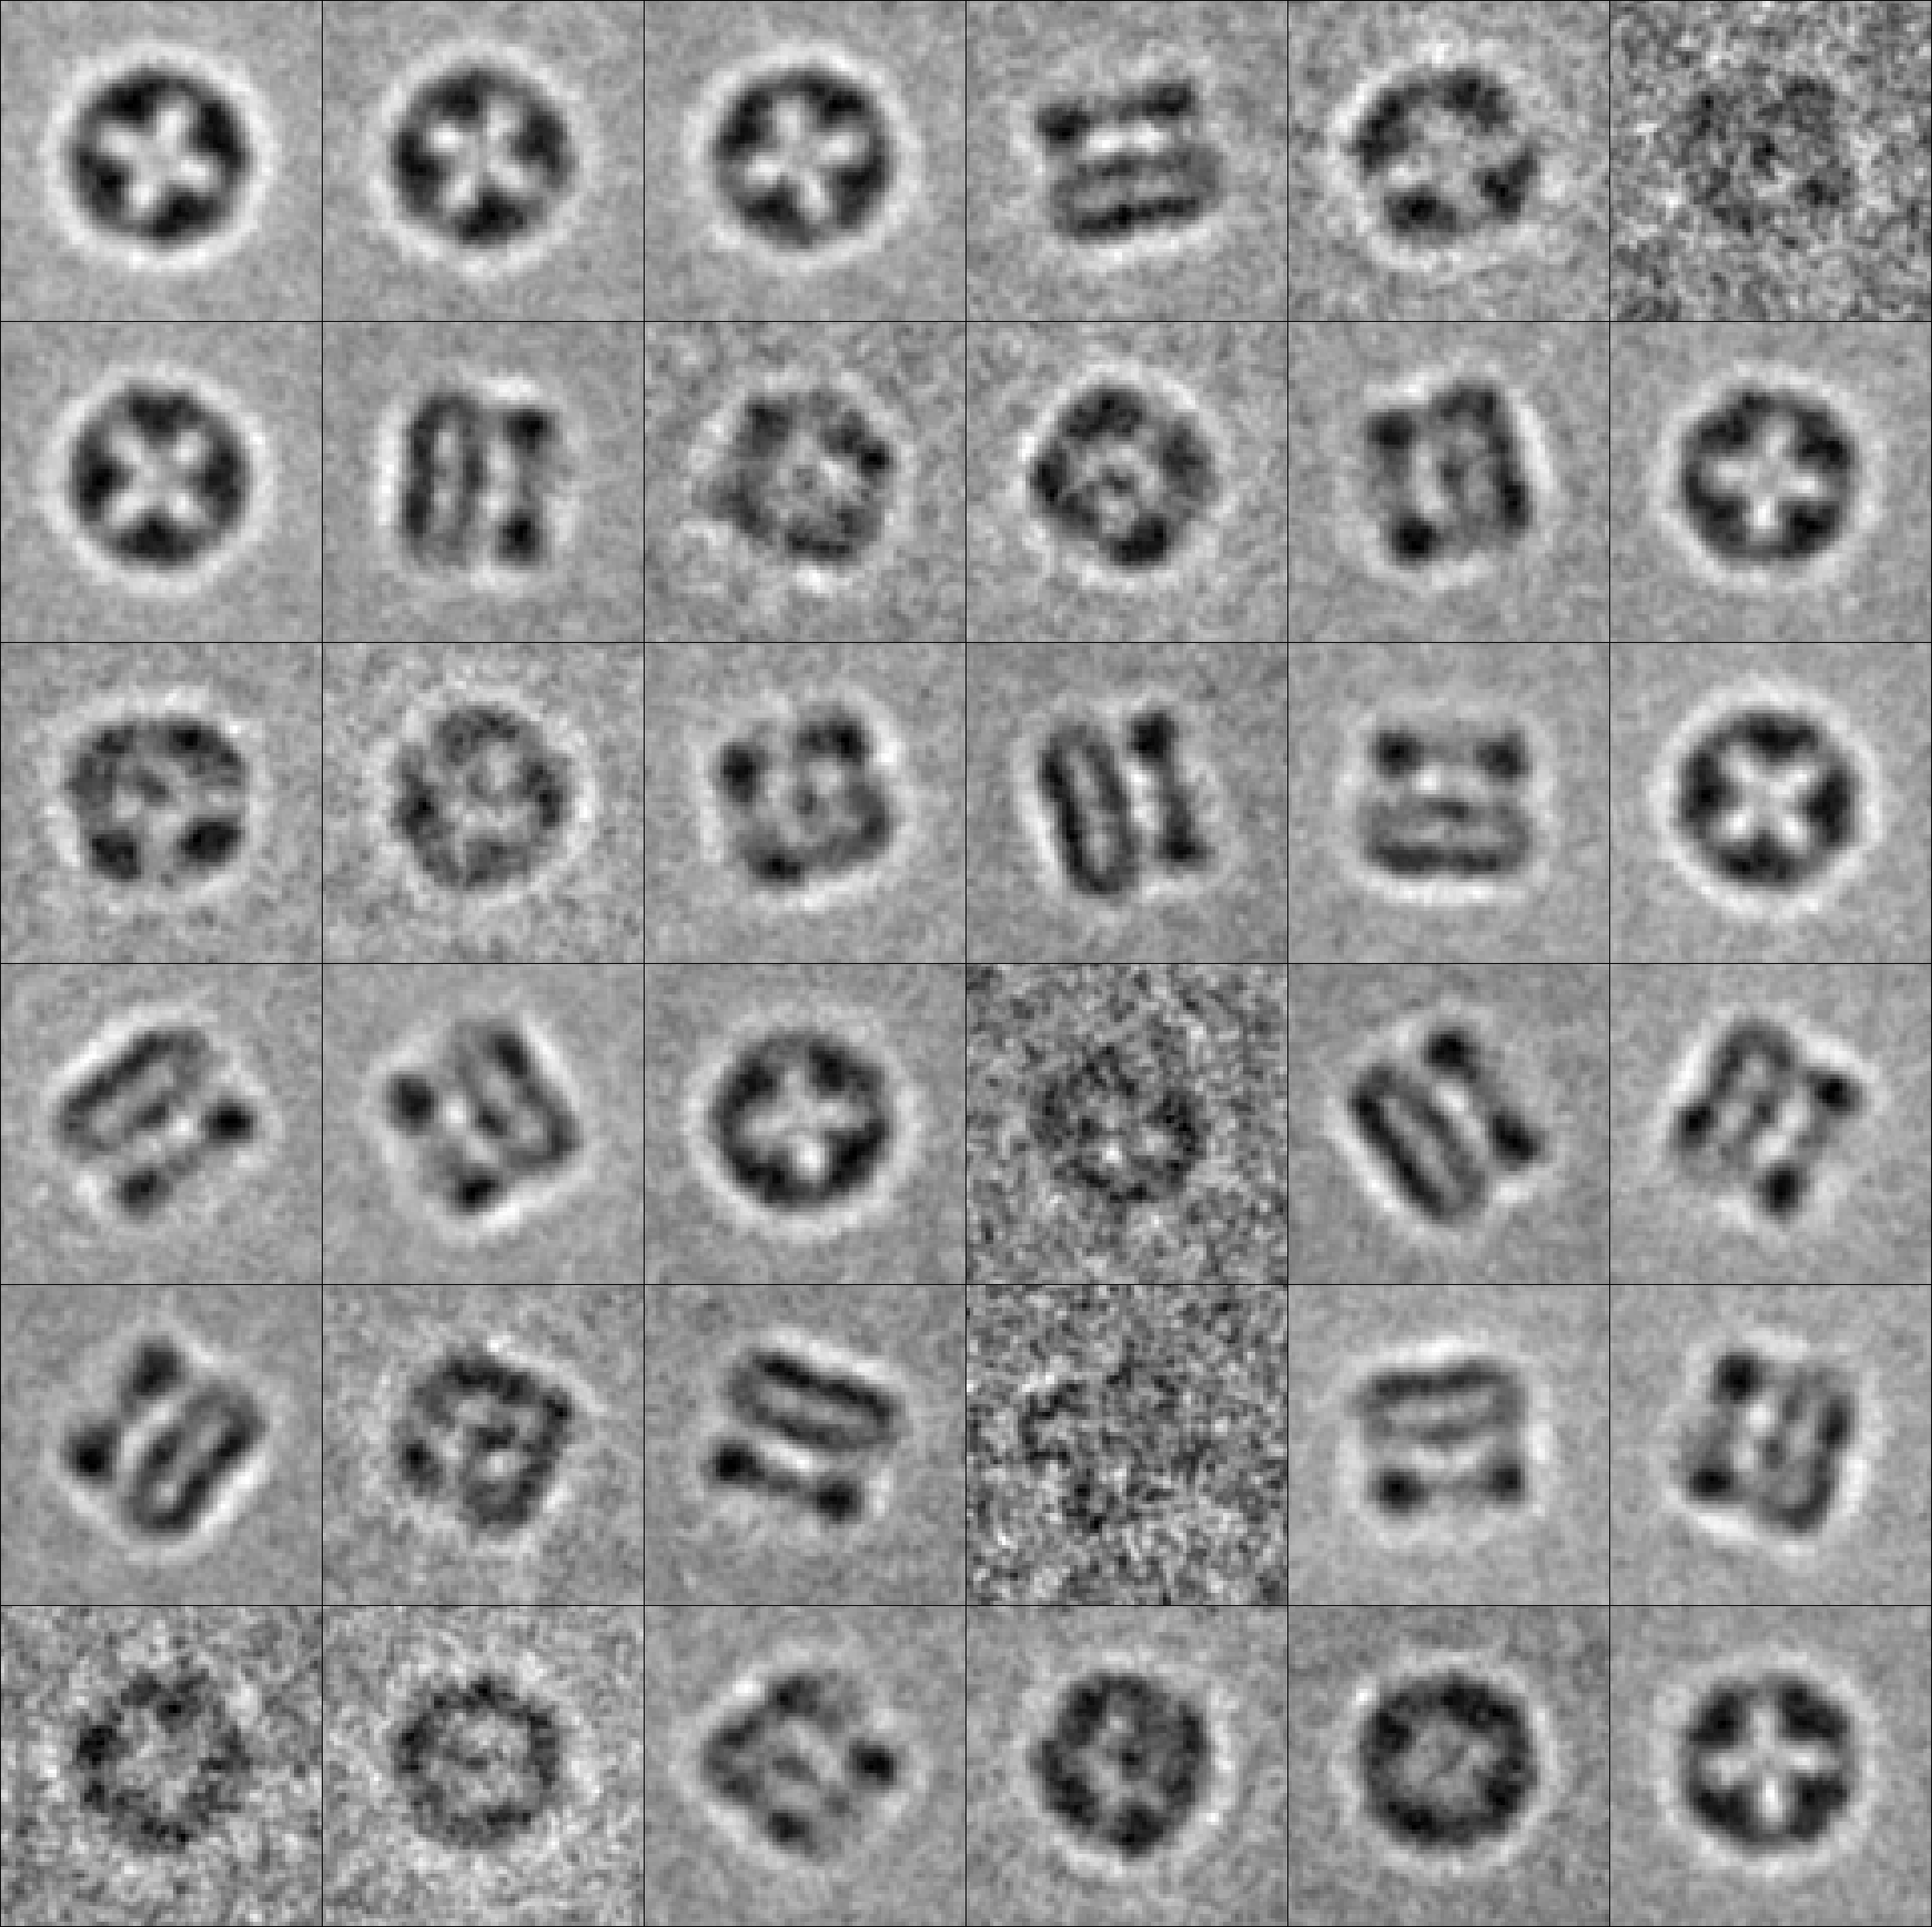
\includegraphics[width=4.8in]{raw_kmeans_36}
\par
Through these graphs, we found that some of the images are too noisy and so we just add the constraints that each of the legal clusters must have enough images(75 or 100) in this cluster.\\
\par
Then we show the images that eliminate the center of the previous clustring step in each example.\\
~\\
This is the image that clustered first time.\\
~\\
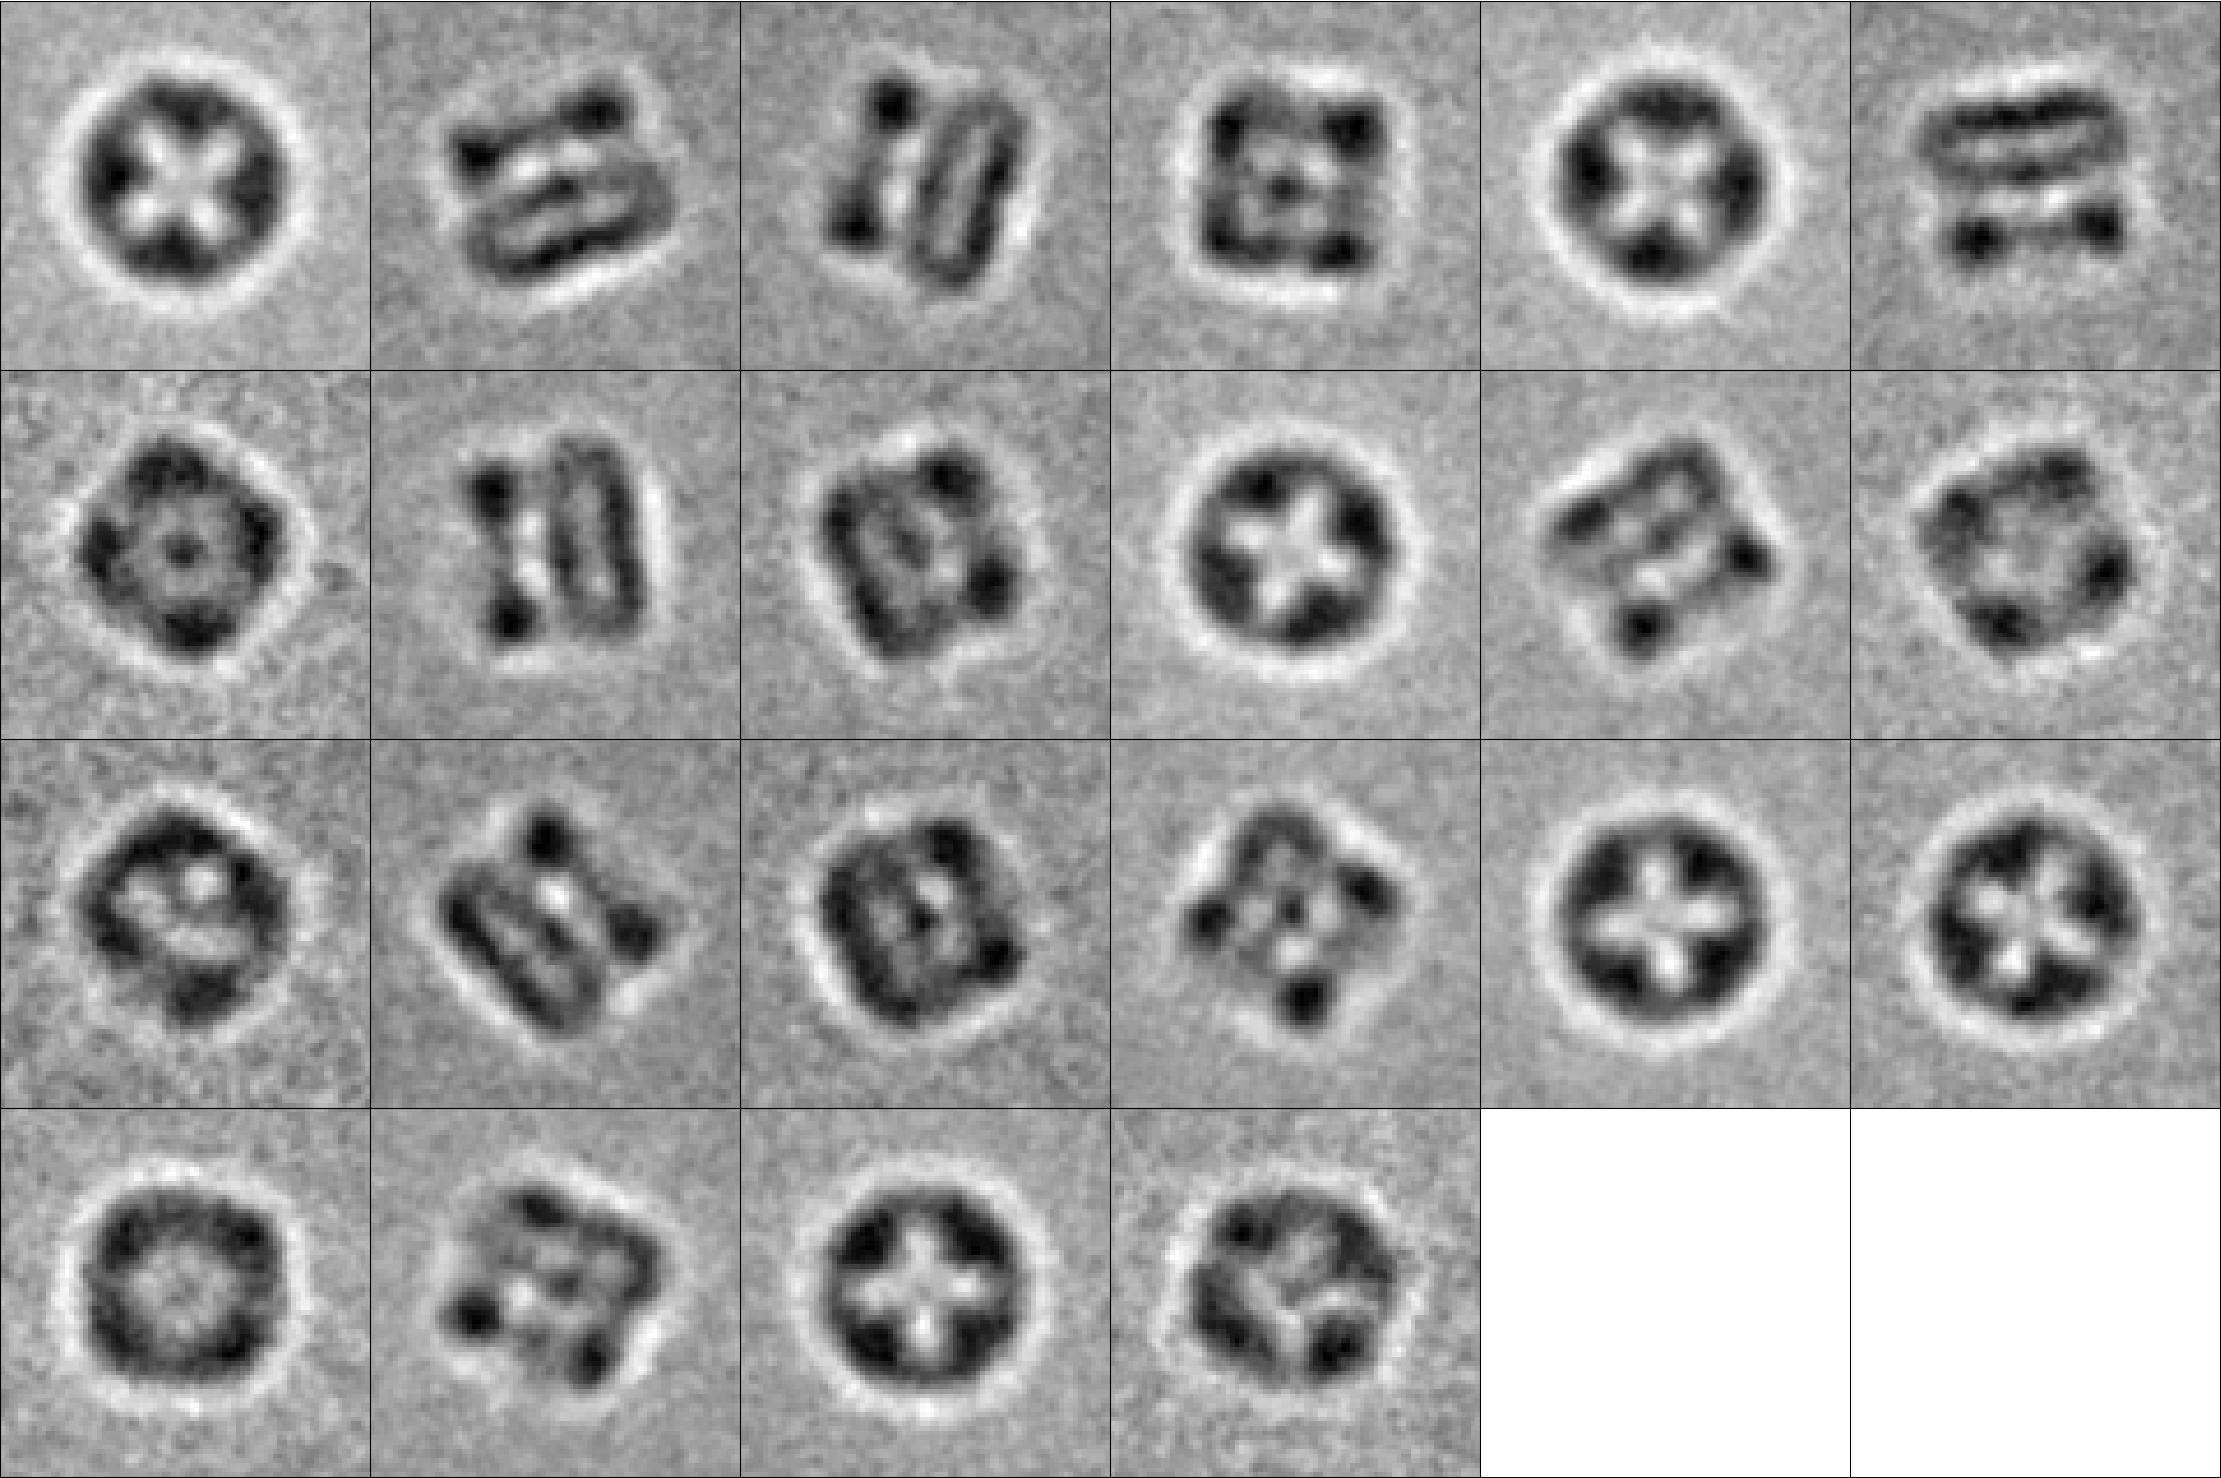
\includegraphics[width=4.8in]{t_first}
~\\
This is the image that we eliminate the clustering center of each example.\\
~\\
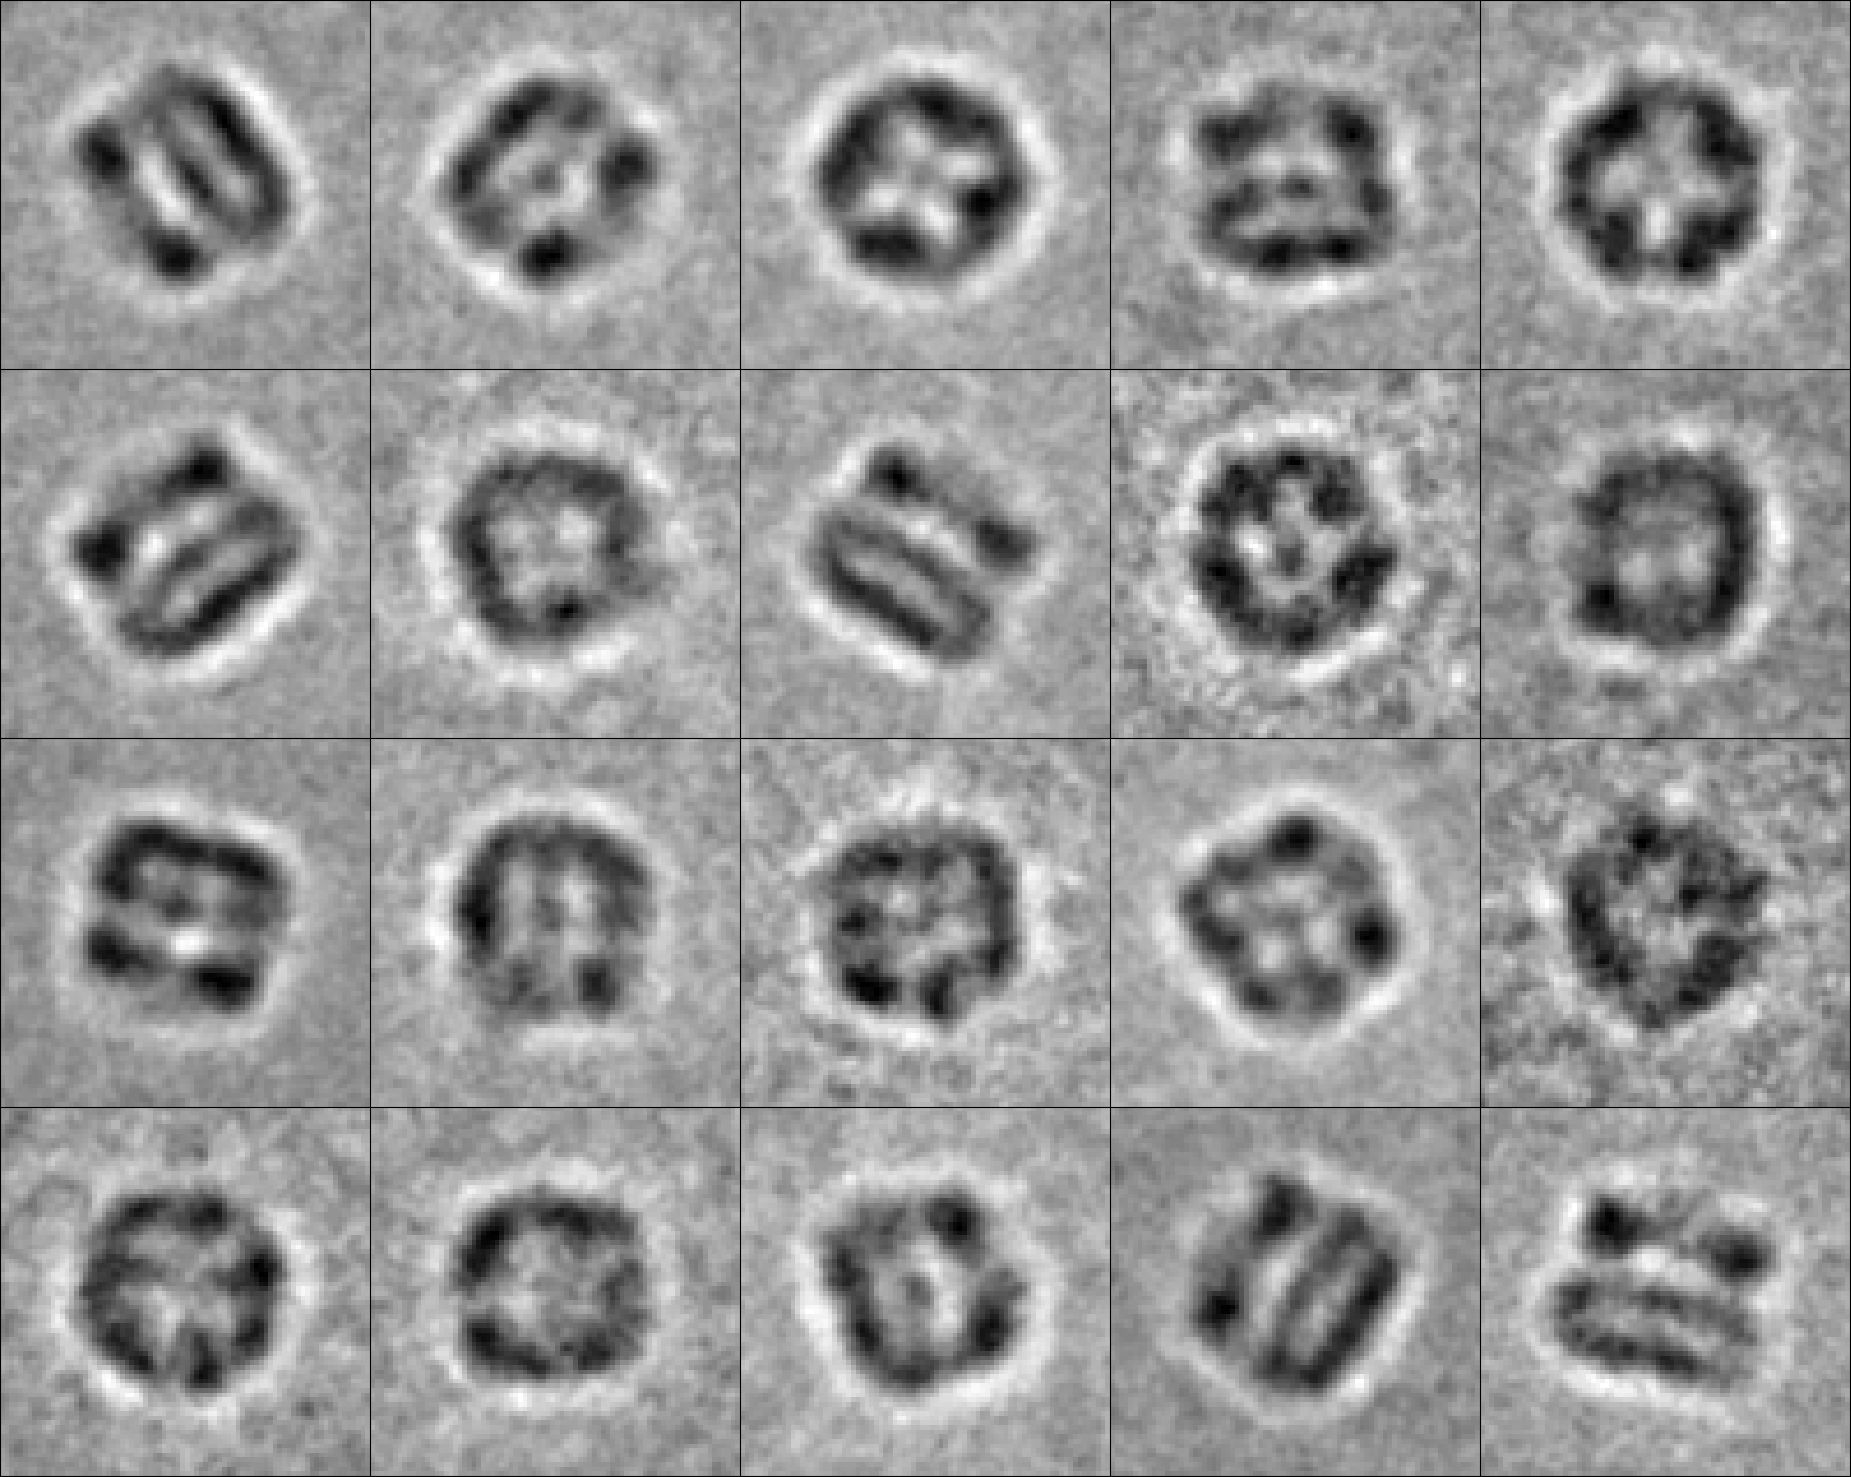
\includegraphics[width=4.8in]{t_second}
~\\
This is the image that we eliminate the clustering center of the first and second time of each example.\\
~\\
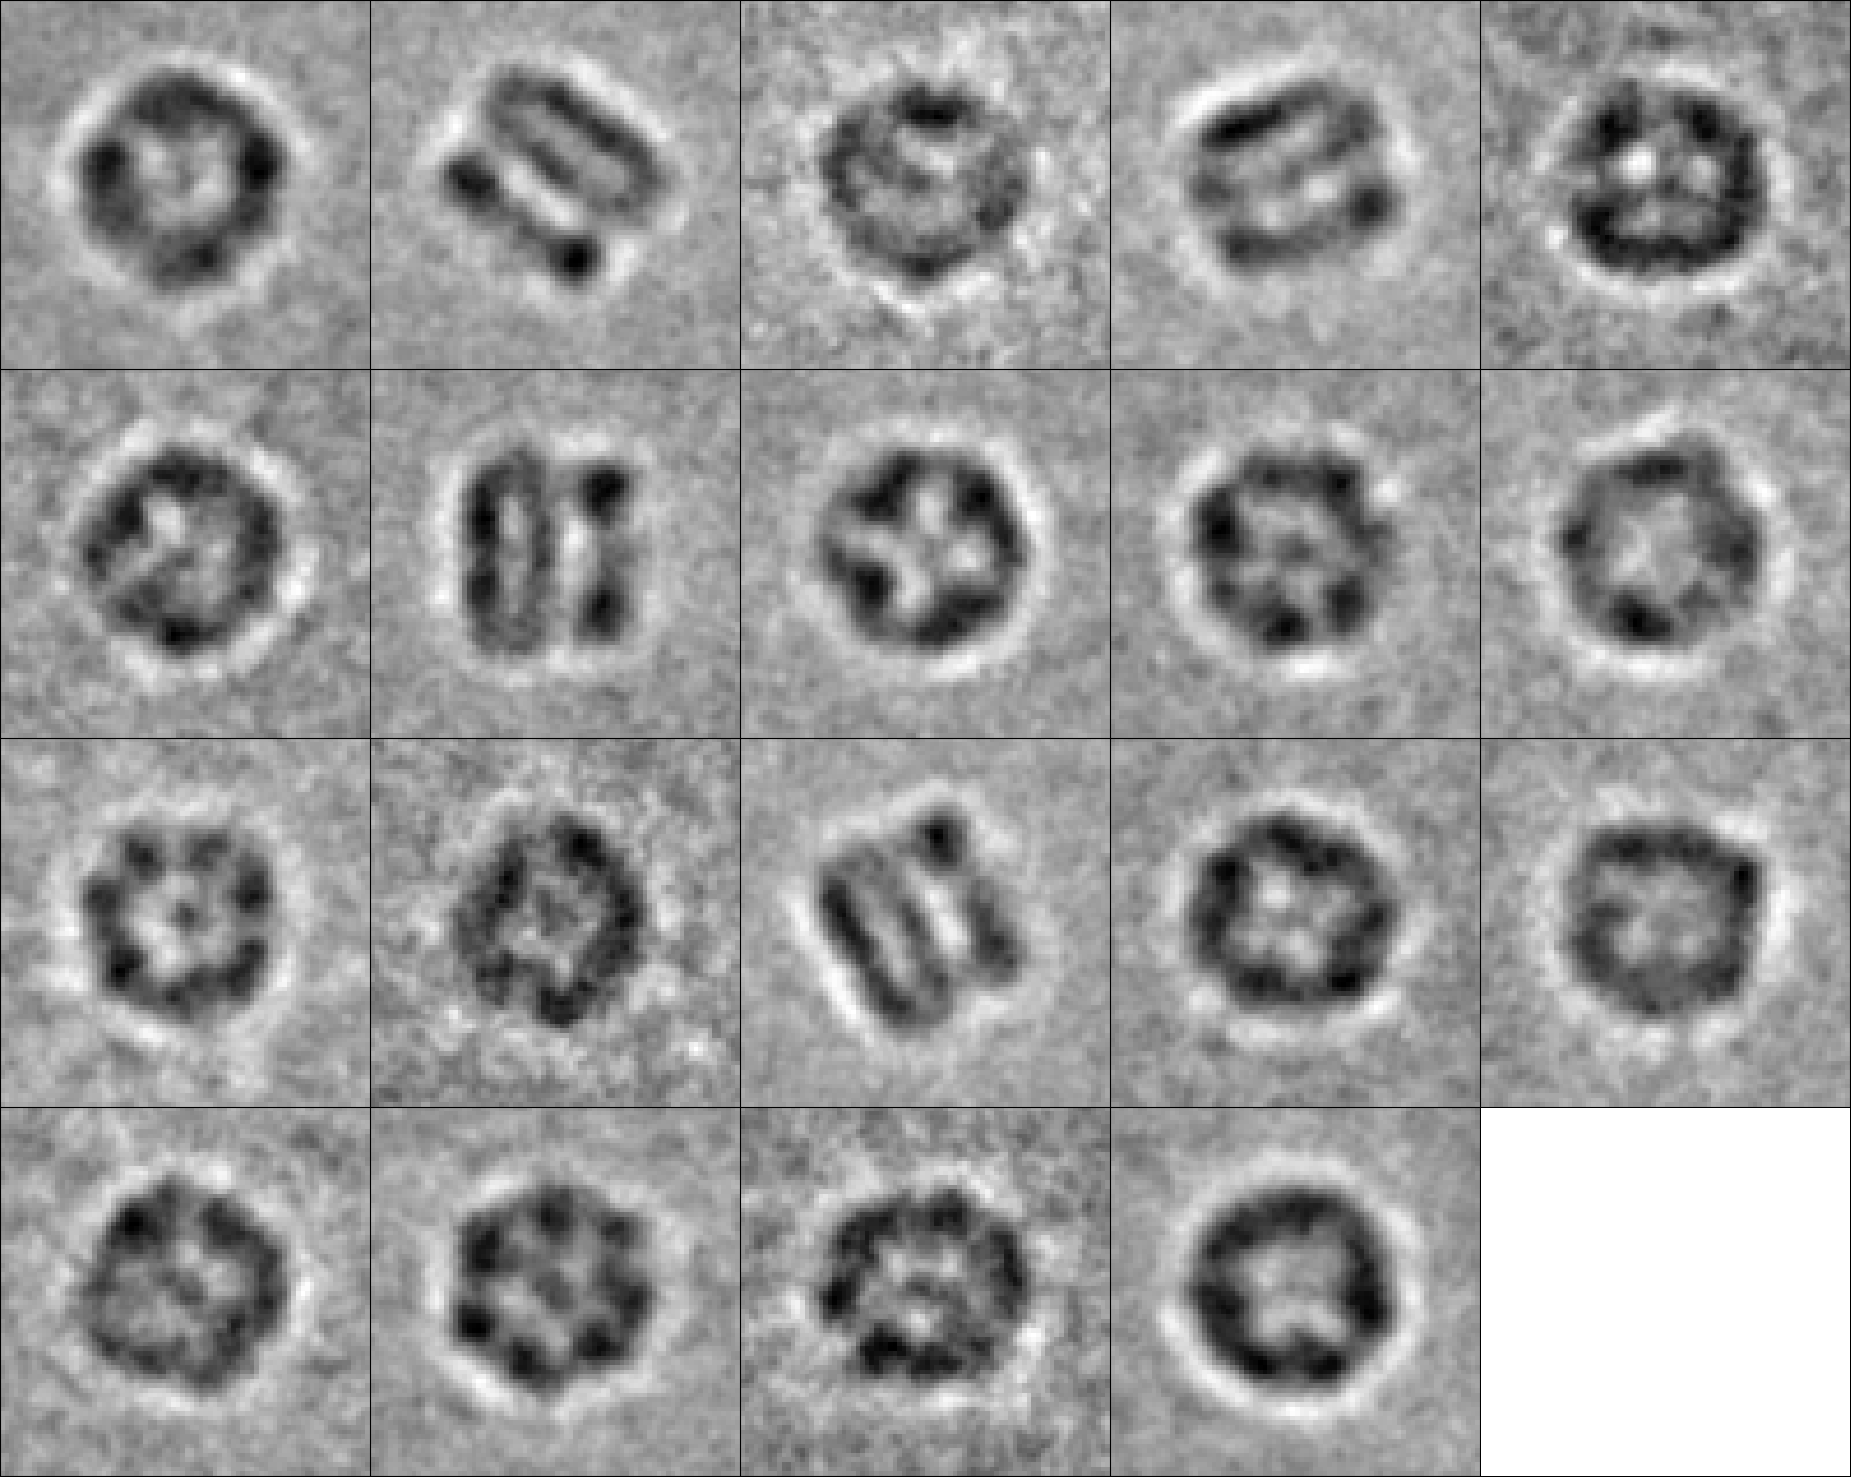
\includegraphics[width=4.8in]{t_third}
~\\

Actually we are very satisfied with these result, but we also want to see whether eleminating the subspace is okey. And we think that the spuared distance of the clustering that eliminating the `principal component' is bounded by no elimination and elimination the subspace, so we just use eliminating the subspace as the final implementation because the elimination of the subspace is faster and easier and can give an upper bound of the method that eliminating just the `principal component' of each cluster.\\
~\\
This is the image of the first clustering.\\
~\\
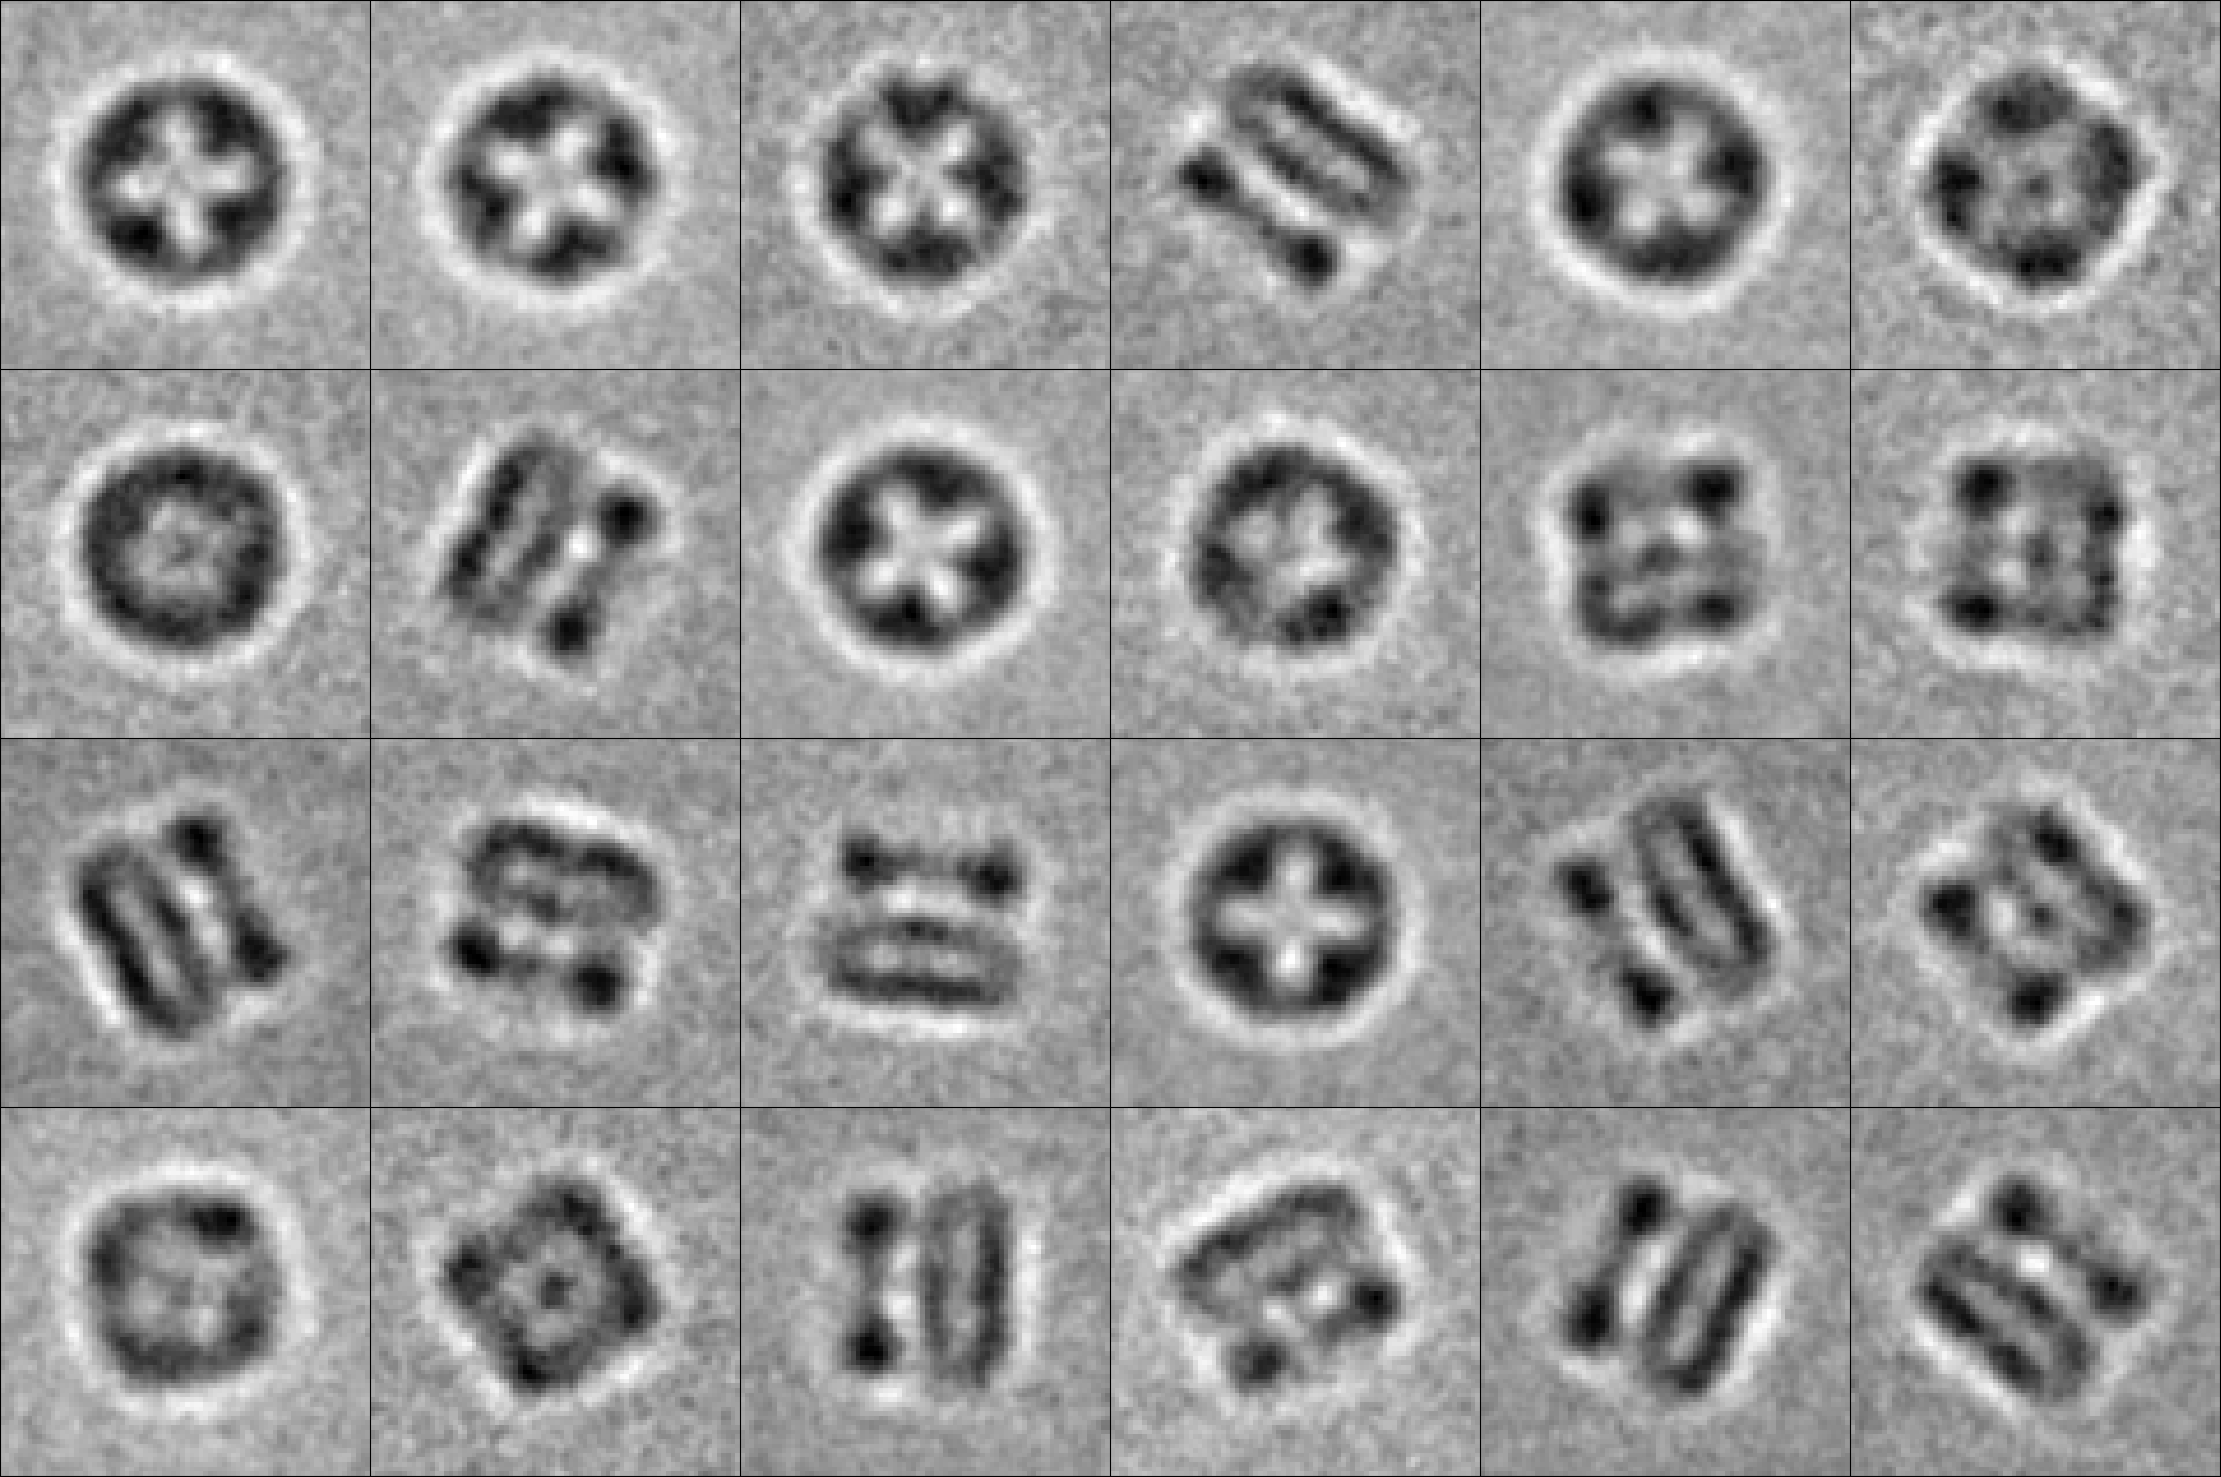
\includegraphics[width=4.8in]{first_clustering}
~\\
This is the image of the second clustering.\\
~\\
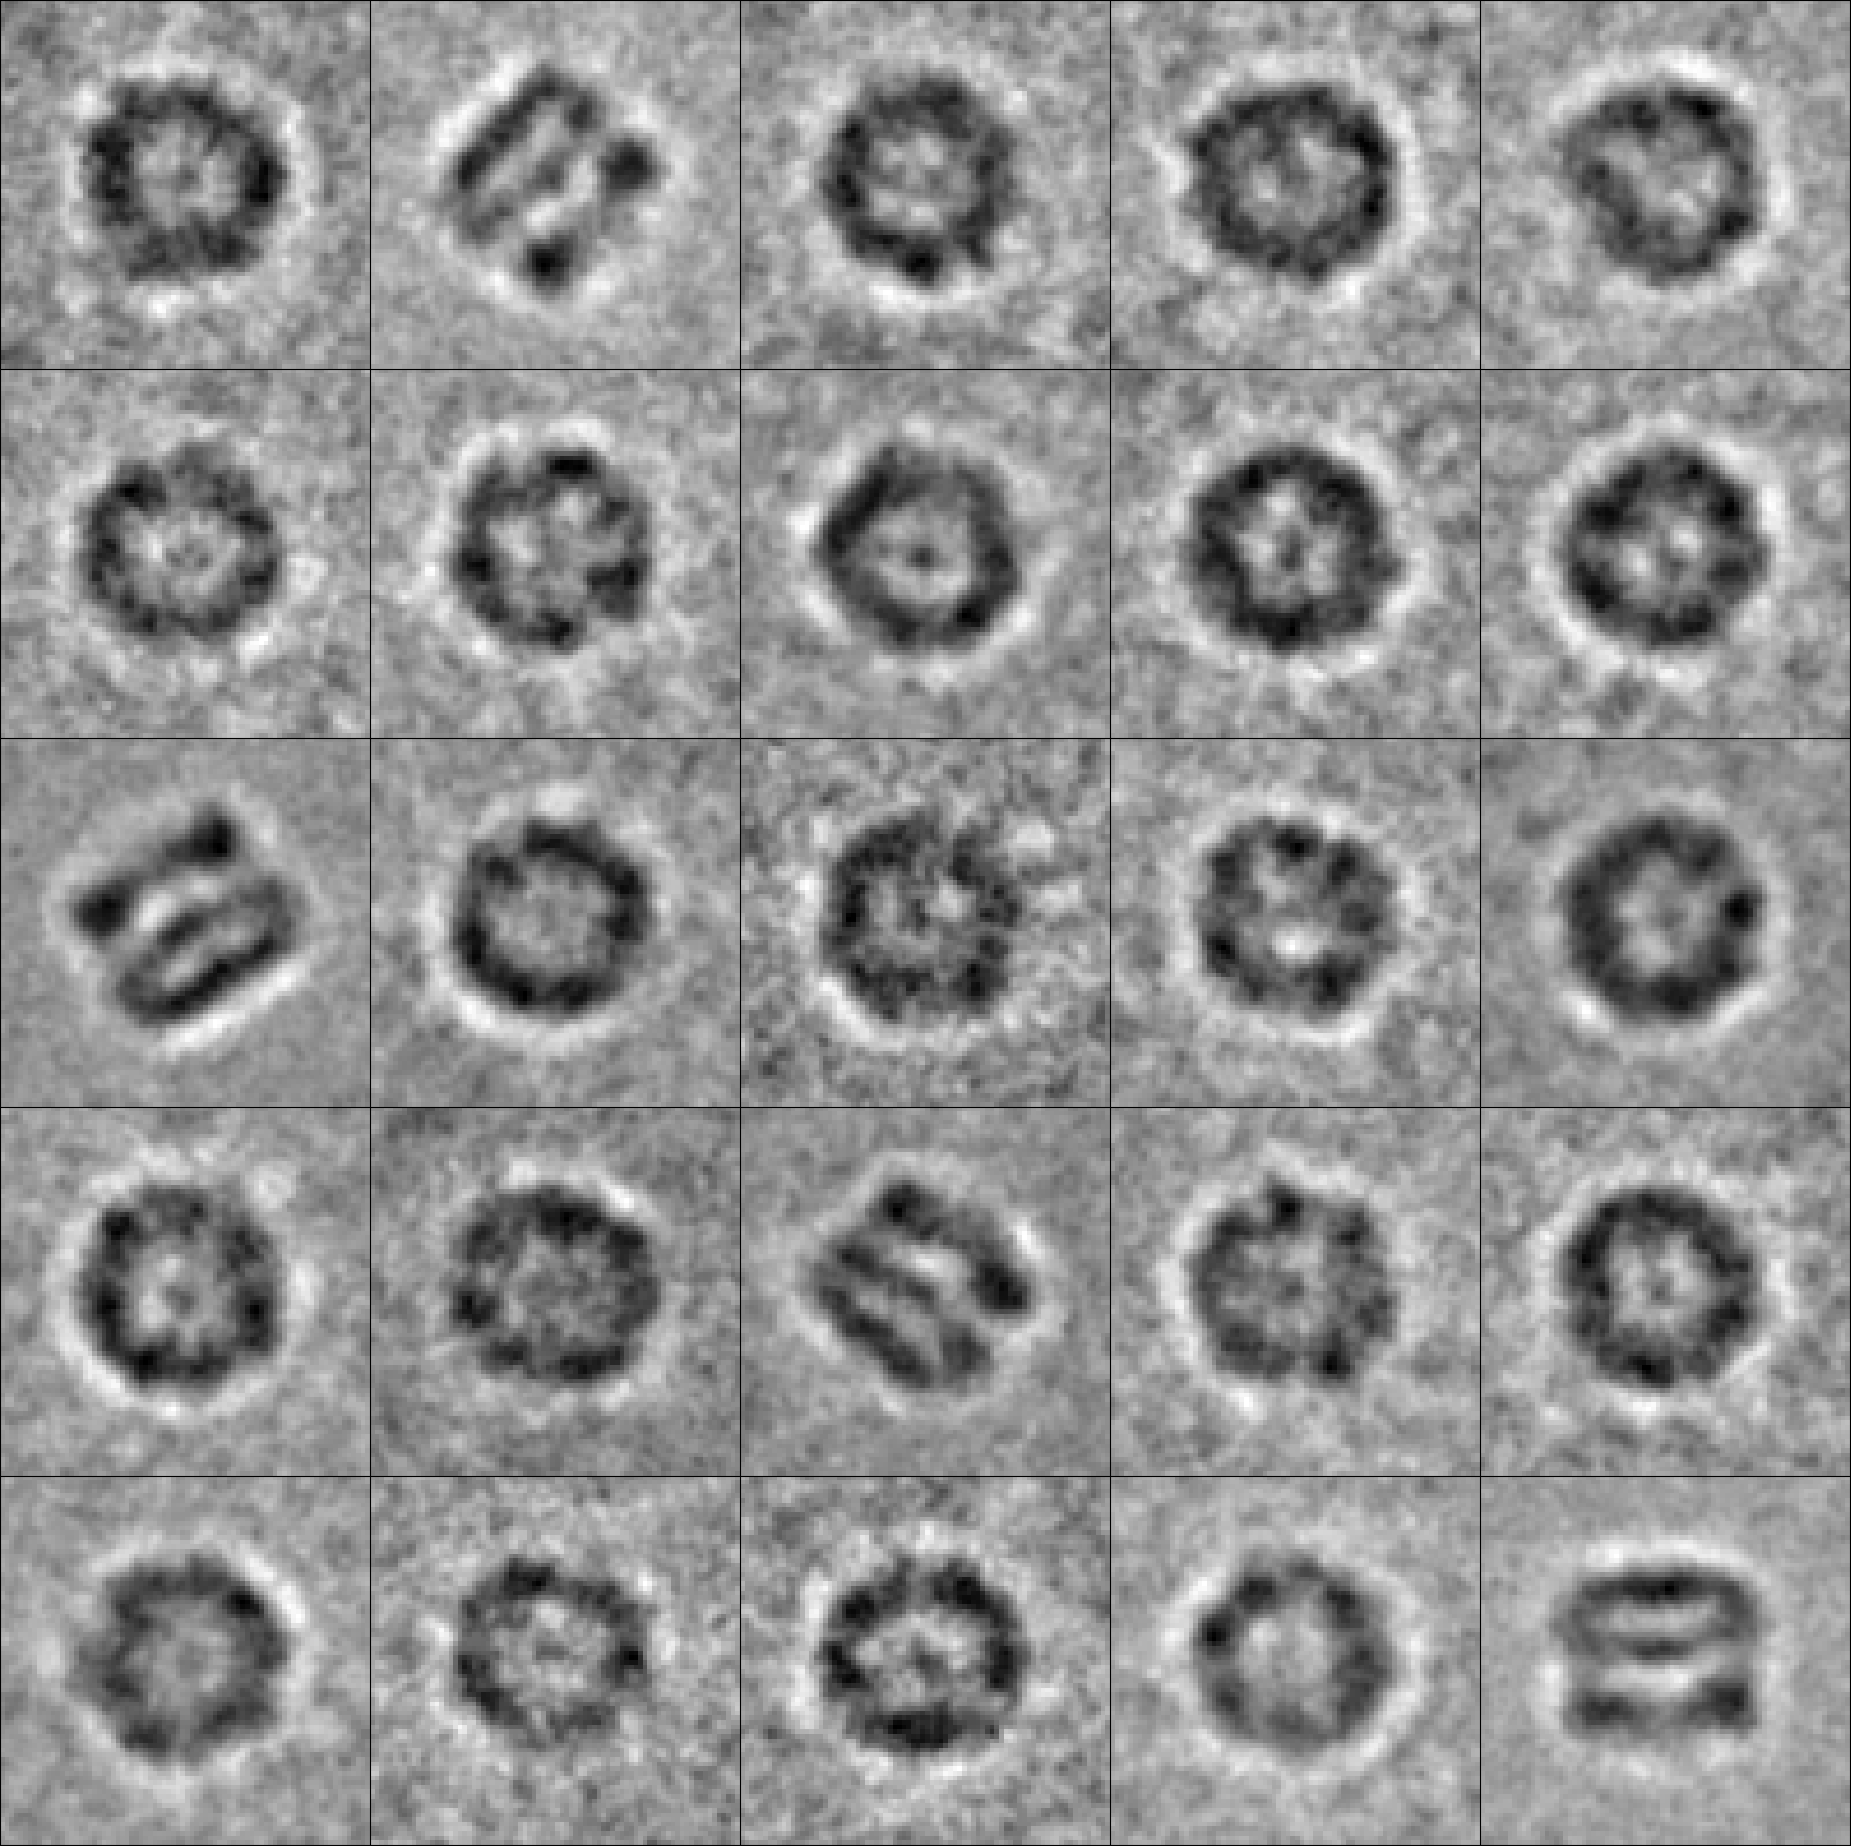
\includegraphics[width=4.8in]{second_clustering}
~\\
We also show the squared distance of the `eliminating subspace cluster'.\\
The mean squared distance of the first clustering phase is 136.72.\\
The mean squared distance of the second clustering phase is 141.42.\\
We see that the mean of the squared distance do not increase so much so we think that the method may be useful to some extent. We also know that these mean squared distance of the clustered data can also bound the version of eliminating the center of each class.\\


\section{Discussion}
First we discuss some of the shortcoming of our implementation or designing of our algorithm.
\begin{enumerate}
\item[1] We think that there may be something wrong with our CTF correction function because the corrected graph isn't change a lot compared with the origianl graph. 
\item[2] We do the down sampling in the image processing step because we do not have enough computational resources. We think that although this step make us easier to do the computation but this will actually lose some mini-structure of the protein.
\item[3] The dimension of each image is 6400(80 by 80) and we just have about 6000-7000 images. The dimension of the image compared with the number of the images is very high. So we should do the PCA or use the autoencoder to reduce the dimension of the data and by the way decrease the noise to some extent, but considering doing the PCA need to generate a 6400 by 6400 matrix and we think that our computer cannot afford this, so we just skip this step in the project.
\end{enumerate}

Then we discuss the contradictory part of our algorithm, that clustering several times after eleminating the subspace of the centers in the previous clustering, theses are our thoughts:
\begin{enumerate}
\item[1] We don't know whether this process make sense or can generate some meaningful images, we just come up with this idea and tried in this project. We just think that it is okey in the low dimension space with very simple data. This method lacks the experiment and theory proof.
\item[2] After the eliminating of the subspace generated by the centers, we cannot see very distinct images, but we think that the mean of the squared distance do not increase a lot, so we believe that these may mean something.
\item[3] Even if the image clustered after eliminating the subspaces do not explain something, this may show some new structure of the data, besides the origianl clustering structure and this may be helpful for the 3d reconstruction.
\end{enumerate}

\section{Contribution of Each Member}
Haoyu Zhao: Writing all the codes and designing the algorithms and learning the CTF correction. Writing part of the reports.
Lukai Li: Studying the CTF correction, collecting the plots in the report and writing part of the report. and do the ppt for the presentation.
Yi Dai: Studying the CTF correction, collecting the plots in the report and writing part of the report. and do the ppt for the presentation.

\section{References}
Haoyu Zhao selected some lectures inteh coursera course about the cryo-EM and discuss with the TA by email.\\
Lukai Li and Yi Dai watch the wikipedia about the CTF.

\end{document}